\section{Use Case Model}
A use case captures how an external actor perceives the system.  In \textbf{MultiModalMan} that actor is the \emph{Player}, who may speak, gesture, or type.

\noindent
\textbf{Primary scenarios}\,: UC1 Start Game, UC2 Select Input Mode, UC3 Guess Letter,  
UC4 Display Word State, UC5 Handle End of Game, UC6 Start New Round.

\begin{table}[h]
\centering
\caption{Figure \ref{fig:uc-diagram} displays the UC1 diagram, which illustrates the primary interactions between the Player and the system.}
\begin{tabularx}{\linewidth}{@{}l l X X@{}}
\toprule
\textbf{ID} & \textbf{Actor} & \textbf{Goal} & \textbf{Outcome} \\
\midrule
UC1 & Player  & Launch the application.                    & Home screen shown\\
UC2 & Player  & Choose voice, gesture, or keyboard.        & Selected channel \\
UC3 & Player\textsuperscript{*} & Guess a letter.          & Word state updated \\
UC4 & System  & Present current word and errors.           & Updated status\\
UC5 & System  & Detect win or loss.                        & Outcome announced\\
\bottomrule
\end{tabularx}
\footnotesize\textsuperscript{*}\,Variants:\ Voice\,+STT,\ Gesture\,+CNN,\ or direct keyboard input.
\end{table}

\begin{figure}[h]
  \centering
  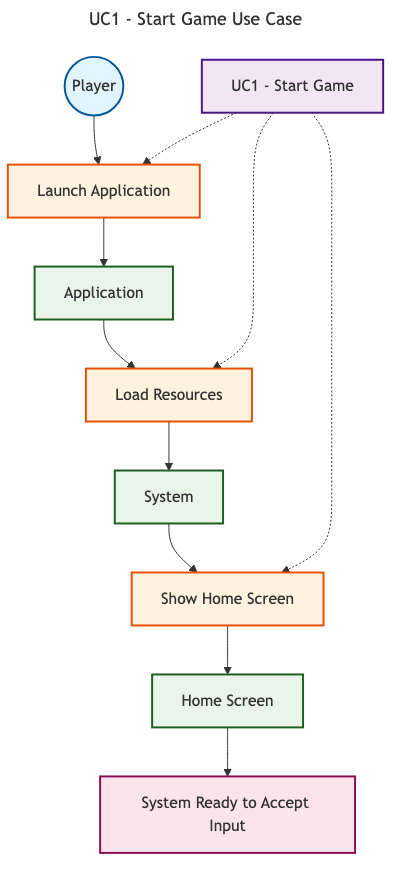
\includegraphics[width=0.3\textwidth]{./images/uc1_start_game.png}
  \caption{Use case diagram for the \textbf{MultiModalMan} game.}
  \label{fig:uc-diagram}
\end{figure}

